\chapter*{Normal Distribution}
Suppose we are in a probability space well approximated by the multivariate normal (Gaussian) distribution of a random variable $x \in \R^n$ with mean $\mu$ and non-singular covariance $\Sigma$:
\marginnote{The $n=1$ example in the introduction is just where where $\mu$ and $\Sigma$ are scalars and $\sigma=\sqrt{\Sigma^{-1}}$.}
\begin{align}
P_{\text{normal}}(x;\mu,\Sigma) &= \frac{e^{-\frac{1}{2}(x-\mu)^T \Sigma^{-1} (x-\mu)}}{\sqrt{(2\pi)^n \det{\Sigma}}}  \,,\\
\intertext{where}
\mu_i &= E(x_i)\,,\\
\intertext{and}
\Sigma_{ij} &= E((x_i-\mu_i)(x_j-\mu_j)) \,.
\end{align}

How lucky is some outcome $x$? From the definition:
\begin{align}
L(x)&=|\Omega(x)|+\frac{1}{2}|\omega(x)| \,,\\
\intertext{where}
\Omega(x) =& \left\{ y \in \R^n \middle| P_{\text{normal}}(y) > P_{\text{normal}}(x) \right\} \\
          =& \left\{ y \in \R^n \middle| |\sqrt{\Sigma^{-1}}(y-\mu)| < |\sqrt{\Sigma^{-1}}(x-\mu)| \right\}
\intertext{and}
\omega(x) =& \left\{ y \in \R^n \middle| |\sqrt{\Sigma^{-1}}(y-\mu)| = |\sqrt{\Sigma^{-1}}(x-\mu)| \right\} \,.
\end{align}
Because $\omega(x)$ has no volume in $\R^n$,
\begin{equation}
|\omega(x)|=\int_{\omega(x)} P_{\text{normal}}(y;\mu,\Sigma) \, dy = 0 \,.
\end{equation}

 So
\begin{align}
L(x) &=|\Omega(x)|\\
     &=\int_{\Omega(x)} P_{\text{normal}}(y;\mu,\Sigma) \,dy\,.
\end{align}

By changing variables to $z=\sqrt{\Sigma^{-1}} (x-\mu)$,
\begin{equation}
L(x) = \int_{|z|<R}  P_{\text{normal}}(z;0,I) \, dz \,,
\end{equation}
where $R = |\sqrt{\Sigma^{-1}} (x-\mu)|$.

This can be evaluated in spherical coordinates:
\begin{align}
\label{eq:normal-luck-as-integral}
L(x)    &=\frac{1}{\sqrt{(2\pi)^{n}}} \int_{0}^{R} \frac{n \pi^{n/2}}{\Gamma(\frac{n}{2}+1)} r^{n-1} e^{-\frac{1}{2} r^2} \, dr \\
    &=\frac{\gamma(n/2,R^2/2)}{\Gamma(n/2)}
\end{align}
The last form uses the lower incomplete gamma function, defined to be
\begin{equation}
\gamma(s,x) = \int_0^{x} t^{s-1} e^{-t} \, dt
\end{equation}
For any value of $n$, but particularly for large values, we find the following approximation to be very good\marginnote{This comes from a taylor expansion of the log of the integrand in (\ref{eq:normal-luck-as-integral}), which is specifically invalid for $n=1$, hence the difference between the general case and the $n=1$ case (\ref{eq:normal-1d-luck}).}:
\begin{equation}
L(x) \approx \frac{1}{2}\left[1+\erf(|\sqrt{\Sigma^{-1}} (x-\mu)|-\sqrt{n-1/2})\right] \,.
\end{equation}
\begin{figure}
  \caption{Exact (blue) vs approximate (red) luck for normal distribution for $n=1$, $10$, and $100$.}
  \centering
    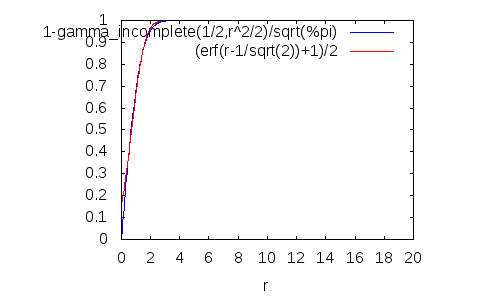
\includegraphics[width=0.75\textwidth]{img/luck1}
    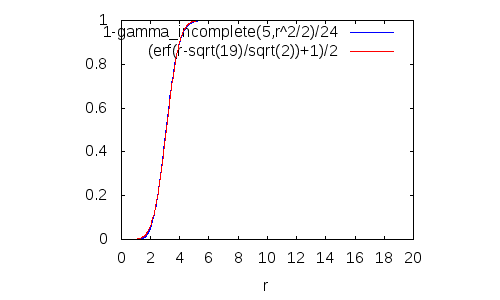
\includegraphics[width=0.75\textwidth]{img/luck10}
    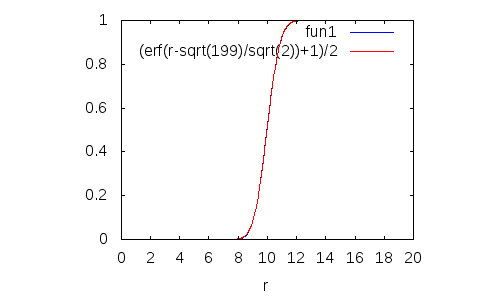
\includegraphics[width=0.75\textwidth]{img/luck100}
\end{figure}

Not only is this result pretty, it is very useful.  Suppose we have distribution parameters $\mu$ and $\Sigma$, and would like to know if they fit actual observations.  A traditional approach requires a large sample to estimate $\mu$ and $\Sigma$, but we don't need this, nor do we need to assume that the distribution is normal.  We just need to ask if the observations are surprising (lucky or unlucky).  In large dimensions, numerical experiments suggest one sample is in most cases sufficient to establish practical certainty (probability of error less than $10^{-15}$).
\begin{table}
\caption{Luck from two randomly generated distributions $\mu^{(x)}$ and $\mu^{(y)}$ uniformly chosen in $[0,1]^{100}$, and $\Sigma^{(x)}, \Sigma^{(y)}$ are transposed squares of random $100 \times 100$ matrices.  In each row, $x$ is  a sample from the $\mu^{(x)},\Sigma^{(x)}$, normal distribution, and $y$ is from the $\mu^{(y)},\Sigma^{(y)}$ distribution.  The actual values of $x$ and $y$ are not given, since they are very large (100 numbers each) and uninteresting.}
\begin{tabular}{|S[table-format=2.10]|S[table-format=2.10]|S[table-format=2.10]|S[table-format=2.10]|}
\multicolumn{1}{c}{$L^{(x)}(x)$} &
\multicolumn{1}{c}{$L^{(y)}(x)$} &
\multicolumn{1}{c}{$L^{(x)}(y)$} &
\multicolumn{1}{c}{$L^{(y)}(y)$} \\
\hline
0.5014172020 & 1.0000000000 & 1.0000000000 & 0.8381802641 \\
0.7314212665 & 1.0000000000 & 1.0000000000 & 0.2392581432 \\
0.9825630339 & 1.0000000000 & 1.0000000000 & 0.2716955127 \\
0.0334550807 & 1.0000000000 & 1.0000000000 & 0.4213206259 \\
0.6894299340 & 1.0000000000 & 1.0000000000 & 0.0744616557 \\
0.7363975937 & 1.0000000000 & 1.0000000000 & 0.2940507284 \\
0.3045212967 & 1.0000000000 & 1.0000000000 & 0.7078490147 \\
0.2311115744 & 1.0000000000 & 1.0000000000 & 0.2903130932 \\
0.5852477199 & 1.0000000000 & 1.0000000000 & 0.6369022028 \\
0.2145529261 & 1.0000000000 & 1.0000000000 & 0.2689897874
\end{tabular}
\end{table}
